%Architecture
\section{Software architecture}
% Mainly Client & server architecture
% advantages for implementation and testing
% advantages for maintenance and evolution

The quality of the overall architecture of a software system is crucial to
any project as it has to perfectly tailor to the need of that particular
project. In fact, a good architecture would not only facilitate the
implementation and testing of the software system but also its maintenance
and evolutions.\newline

Great attention was thus given to the choice of a software architecture
perfectly tailoring the need of our project and after extensively analyzing
the various architectures that exist, we settled on a 3-tier client-server
architecture. \newline

\begin{figure}[H]
	\centering
	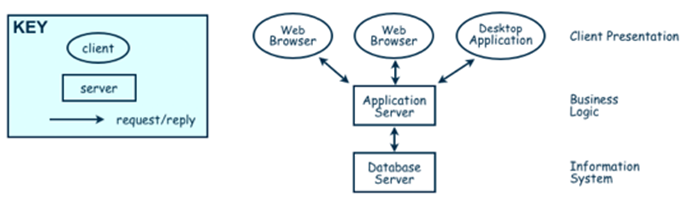
\includegraphics[width=0.8\linewidth]{ClientServerArchitecture.png}
	\caption{3-tier client-server architecture diagram}
    \label{djangoclientserver}
\end{figure}

This easily scalable architecture is perfectly tailored to the
implementation of website in general as it allows multiple request to reach
an application server without any loss. The transport of request/responses
between the client browser and our server will be guaranteed by the http(s)
protocol. \newline

The application server which processes the various requests of the clients
will then access/update the databases, following the need it faces. As this
database connexion must be lossless to avoid critical errors, we will make
use of the TCP protocol to guarantee that everything comes through without
losses. \newline

This allows for a simple yet scalable architecture that is highly evolutive.
In fact, switching to a 4-tier or 5-tier architecture of the same model
remains possible with minor changes if the needs arise. Those n-tier
architecture can contain additional layer proposing various utilities such
as load balancing to redirect the traffic between application server or
small additional servers that are tailored to process a certain part of the
request. \newline

As you can see, this type of architecture is perfectly suited for this
project as everything can be handled through request, whether forms, searches
or any other aspects of the program we have to code. This type architecture will
also allow us to easily set up backup databases that would preserve the
data in case of failure. \newline

In short this architecture will allow us to implement soon a working
version of the project while using only the crucial component of the n-tier
architecture. All while conserving the opportunity to easily scale up
should the need arise. We believe that this scalable architecture will not
only fulfil the current need of the clients for a working website but also
their eventual future need in terms of scaling up their processing power to
support more traffic.
